\documentclass[12pt]{article}
\usepackage{amsfonts}
\usepackage{fancyhdr}
\usepackage[a4paper, top=2.5cm, bottom=2.5cm, left=2.2cm, right=2.2cm]{geometry}
\usepackage{times}
\usepackage{amsmath}
\usepackage{changepage}
\usepackage{amssymb}
\usepackage{graphicx}%
\setcounter{MaxMatrixCols}{30}
\newtheorem{theorem}{Theorem}
\newtheorem{acknowledgement}[theorem]{Acknowledgement}
\newtheorem{algorithm}[theorem]{Algorithm}
\newtheorem{axiom}{Axiom}
\newtheorem{case}[theorem]{Case}
\newtheorem{claim}[theorem]{Claim}
\newtheorem{conclusion}[theorem]{Conclusion}
\newtheorem{condition}[theorem]{Condition}
\newtheorem{conjecture}[theorem]{Conjecture}
\newtheorem{corollary}[theorem]{Corollary}
\newtheorem{criterion}[theorem]{Criterion}
\newtheorem{definition}[theorem]{Definition}
\newtheorem{example}[theorem]{Example}
\newtheorem{exercise}[theorem]{Exercise}
\newtheorem{lemma}[theorem]{Lemma}
\newtheorem{notation}[theorem]{Notation}
\newtheorem{problem}[theorem]{Problem}
\newtheorem{proposition}[theorem]{Proposition}
\newtheorem{remark}[theorem]{Remark}
\newtheorem{solution}[theorem]{Solution}
\newtheorem{summary}[theorem]{Summary}
\usepackage{enumitem}
\usepackage[utf8]{inputenc}
\newenvironment{proof}[1][Proof]{\textbf{#1.} }{\ \rule{0.5em}{0.5em}}
\usepackage{tikz}
\usepackage{graphicx}
\usepackage{wrapfig}
\usepackage{float}
\usepackage{datetime}
\newdateformat{specialdate}{\twodigit{\THEDAY}.\twodigit{\THEMONTH}.\THEYEAR}


\newcommand{\Q}{\mathbb{Q}}
\newcommand{\R}{\mathbb{R}}
\newcommand{\C}{\mathbb{C}}
\newcommand{\Z}{\mathbb{Z}}

\begin{document}
	
	\title{1. Übung}
	\author{Timo Bergerbusch 344408 \& Marc Burian 344300}
	\date{\specialdate\today}
	\maketitle
	
	
	\section{Aufgabe 1}
	\subsection{a)}
	\begin{figure}[H]
		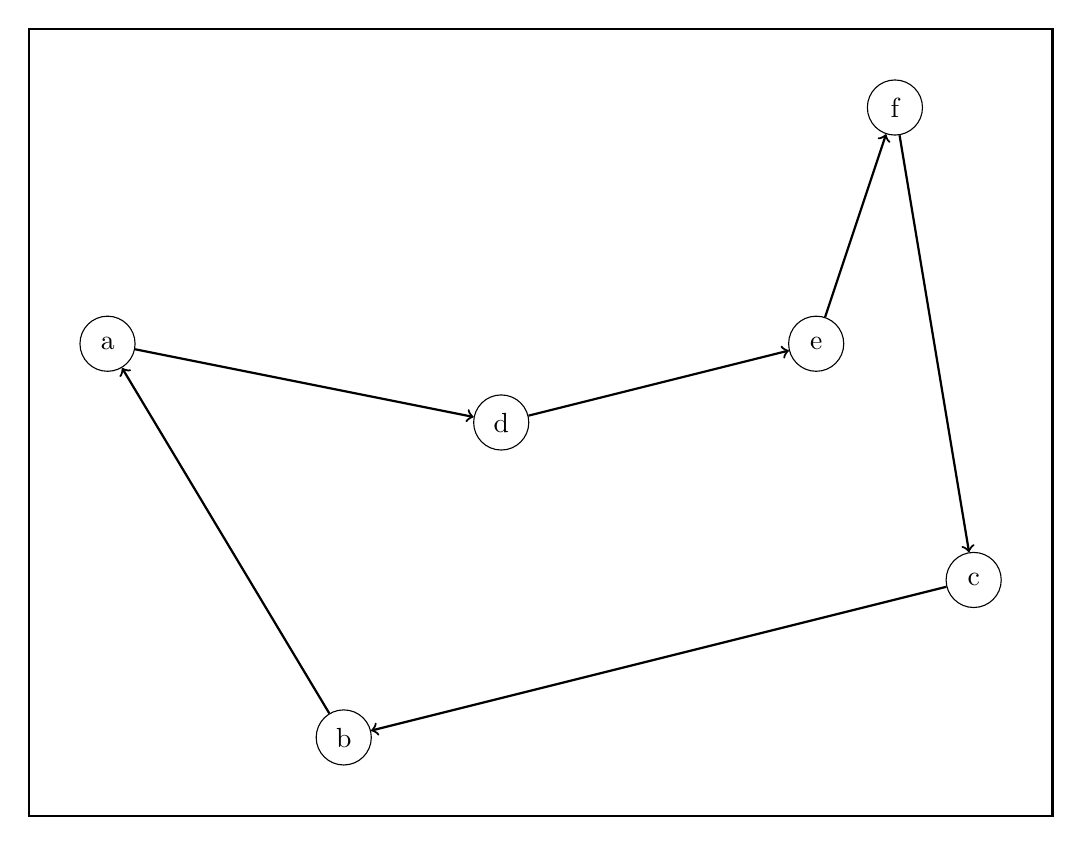
\begin{tikzpicture}
		\begingroup
		\draw[thick] (0,0) rectangle (13,10);
		
		\node[draw, circle, fill=white,inner sep=2pt,minimum size=0.7cm] (a) at (1, 6) {a};
		\node[draw, circle, fill=white,inner sep=2pt,minimum size=0.7cm] (b) at (4, 1) {b};
		\node[draw, circle, fill=white,inner sep=2pt,minimum size=0.7cm] (c) at (12, 3) {c};
		\node[draw, circle, fill=white,inner sep=2pt,minimum size=0.7cm] (d) at (6, 5) {d};
		\node[draw, circle, fill=white,inner sep=2pt,minimum size=0.7cm] (e) at (10, 6) {e};
		\node[draw, circle, fill=white,inner sep=2pt,minimum size=0.7cm] (f) at (11, 9) {f};
		
		
		\draw[->, thick] (a) -- (d);
		\draw[->, thick] (d) -- (e);
		\draw[->, thick] (e) -- (f);
		\draw[->, thick] (f) -- (c);
		\draw[->, thick] (c) -- (b);
		\draw[->, thick] (b) -- (a);
		\endgroup
		\end{tikzpicture}		
	\end{figure}
	
	\subsection{b)}
	\begin{figure}[H]
		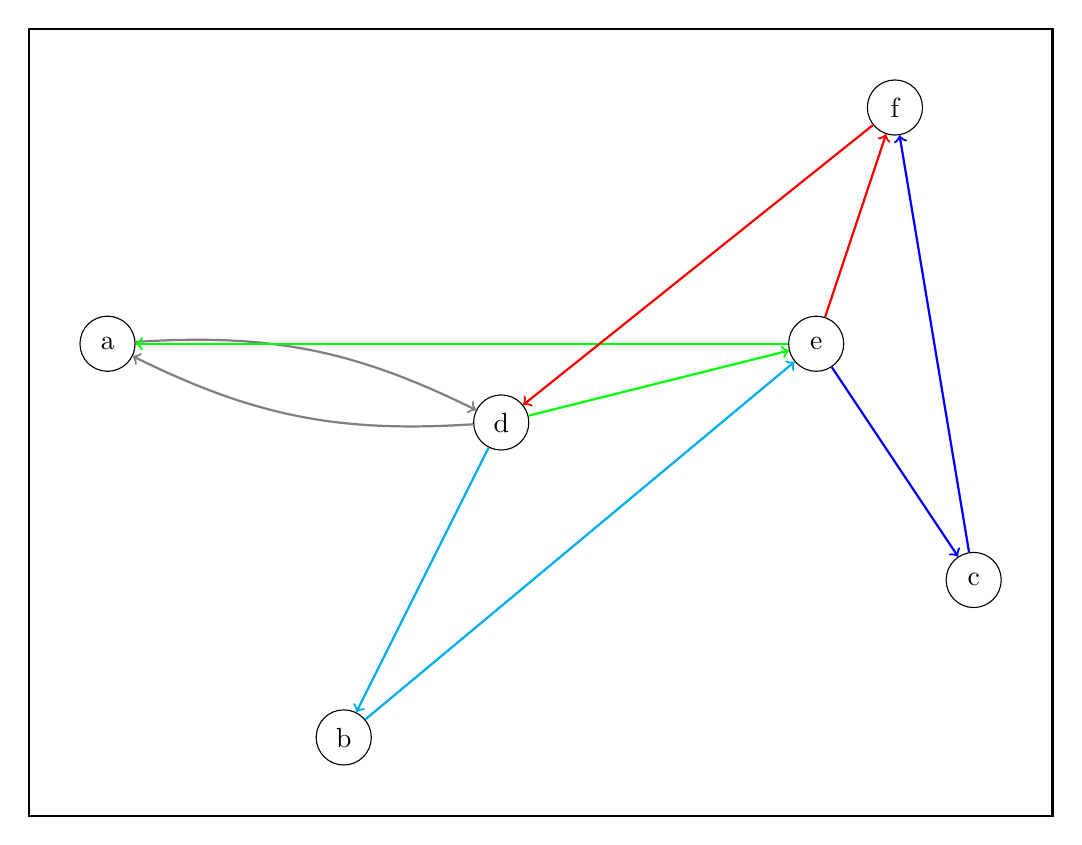
\begin{tikzpicture}
		\begingroup
		\draw[thick] (0,0) rectangle (13,10);
		
		\node[draw, circle, fill=white,inner sep=2pt,minimum size=0.7cm] (a) at (1, 6) {a};
		\node[draw, circle, fill=white,inner sep=2pt,minimum size=0.7cm] (b) at (4, 1) {b};
		\node[draw, circle, fill=white,inner sep=2pt,minimum size=0.7cm] (c) at (12, 3) {c};
		\node[draw, circle, fill=white,inner sep=2pt,minimum size=0.7cm] (d) at (6, 5) {d};
		\node[draw, circle, fill=white,inner sep=2pt,minimum size=0.7cm] (e) at (10, 6) {e};
		\node[draw, circle, fill=white,inner sep=2pt,minimum size=0.7cm] (f) at (11, 9) {f};
		
		\draw[thick, ->,gray, bend angle=15, bend left] (a) to (d);
		\draw[thick, ->,gray, bend angle=15, bend left] (d) to (a);
		
		\draw[thick, ->,green] (d) to (e);
		\draw[thick, ->,green] (e) to (a);
		
		\draw[thick, ->,red] (e) to (f);
		\draw[thick, ->,red] (f) to (d);
		
		\draw[thick, ->,blue] (e) to (c);
		\draw[thick, ->,blue] (c) to (f);
		
		\draw[thick, ->,cyan] (d) to (b);
		\draw[thick, ->,cyan] (b) to (e);
		\endgroup
		\end{tikzpicture}	
	\end{figure}
		\begin{enumerate}
			\item[\color{gray}1] starte mit: (a,d), (d,a)
			\item[\color{green}2] nächster Knoten: e mit 41 über d \\
				a$\rightarrow$e$\rightarrow$d$\rightarrow$a: 90 + 41 + 51= 182 \\
				a$\rightarrow$d$\rightarrow$e$\rightarrow$a: 51 + 41 + 90 = 182\\
				$\Rightarrow$ lösche (d,a) und füge (d,e)(e,a) hinzu
			\item[\color{red}3] nächster Knoten: f mit 32 über e \\
			%TODO: a->e nicht e->d%
				a$\rightarrow$f$\rightarrow$e$\rightarrow$...: 104+32=136\\
				e$\rightarrow$f$\rightarrow$d$\rightarrow$...: 32+64=96\\
				$\Rightarrow$ lösche (e,d) und füge (e,f),(f,d) hinzu
			\item[\color{blue}4] nächster Knote: c mit 36 über e \\
				d$\rightarrow$c$\rightarrow$e$\rightarrow$...: 63+36=99\\
				e$\rightarrow$c$\rightarrow$f$\rightarrow$...: 36+61=97\\
				$\Rightarrow$ lösche (e,f) und füge (e,c),(c,f) hinzu
			\item[\color{cyan}5] nächster Knoten: b mit 45 über d \\
				a$\rightarrow$b$\rightarrow$d$\rightarrow$...: 58+45=103\\
				d$\rightarrow$b$\rightarrow$e$\rightarrow$...: 45+78=123\\
				$\Rightarrow$ lösche (d,e) und füge (d,b),(b,e) hinzu
		\end{enumerate}	
		
		\begin{figure}[H]
			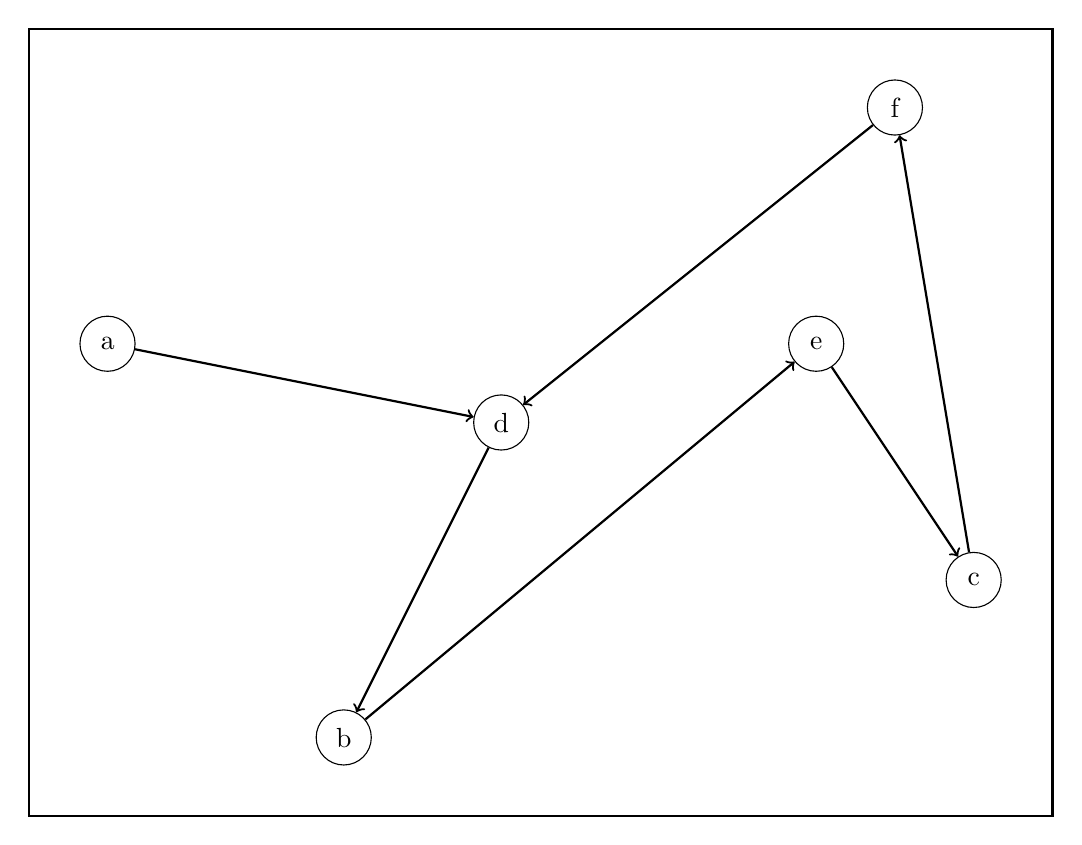
\begin{tikzpicture}
			\begingroup
			\draw[thick] (0,0) rectangle (13,10);
			
			\node[draw, circle, fill=white,inner sep=2pt,minimum size=0.7cm] (a) at (1, 6) {a};
			\node[draw, circle, fill=white,inner sep=2pt,minimum size=0.7cm] (b) at (4, 1) {b};
			\node[draw, circle, fill=white,inner sep=2pt,minimum size=0.7cm] (c) at (12, 3) {c};
			\node[draw, circle, fill=white,inner sep=2pt,minimum size=0.7cm] (d) at (6, 5) {d};
			\node[draw, circle, fill=white,inner sep=2pt,minimum size=0.7cm] (e) at (10, 6) {e};
			\node[draw, circle, fill=white,inner sep=2pt,minimum size=0.7cm] (f) at (11, 9) {f};
			
			\draw[thick, ->] (a) to (d);		
			\draw[thick, ->] (f) to (d);
			\draw[thick, ->] (e) to (c);
			\draw[thick, ->] (c) to (f);
			\draw[thick, ->] (d) to (b);
			\draw[thick, ->] (b) to (e);
			\endgroup
			\end{tikzpicture}	
		\end{figure}
\end{document}


















